% Copyright 2007 by Till Tantau
%
% This file may be distributed and/or modified
%
% 1. under the LaTeX Project Public License and/or
% 2. under the GNU Public License.
%
% See the file doc/licenses/LICENSE for more details.


\lecture[11]{Comparing two samples}{lecture-text}

\subtitle{hypothesis testing, and the $t$ statistic}

\date{2 March 2015}

% pp. 218-(242?)


\begin{document}

\begin{frame}
  \maketitle
\end{frame}


\begin{frame}\frametitle<presentation>{Outline}
  \tableofcontents
\end{frame}


\section{Hypothesis testing}

%%%%%%
\begin{frame}{The goal}

    You have measurements from two groups of samples:
    \begin{itemize}
        \item case/control
        \item treatment/control
        \item red/green
        \item (etcetera)
    \end{itemize}

    \vspace{2em}

    They have different \alert{sample} means:
    \[  \bar y_1 > \bar y_2 . \]
    Do we believe the groups are different?

    \vspace{2em}
    \pause

    \begin{block}{First approach:}
      \begin{itemize}
        \item If the label has no effect,
        \item we can imagine the samples are from the \alert{same population}, so
        \item \structure{randomizing} the \alert{group labels}
          estimates how big a difference $|\bar y_1 - \bar y_2|$ is expected 
          due to random chance.
      \end{itemize}
    \end{block}

\end{frame}


%%%%%
\begin{frame}{Example: }

    Flexibility (in cm):  
    \begin{center}
      \begin{tabular}{cYY}
        & Aerobics & Dance \\
       \hline
       & 38  & 48 \\
       & 45  & 59 \\
       & 58  & 61 \\
       & 64  & \\
       \hline
       mean & 51.25 & 56.00 \\
     \end{tabular}
   \end{center}
     A 10\% difference!  Do we believe it?

     \vspace{2em}

     \pause

     \structure{Proportion of} rearrangements with
     \[
         | \bar y_1 - \bar y_2 | > |51.25-56.00| = 4.75
     \]
     is $20/35 = 0.57$.

     \vspace{1em}
     \pause
     This is \alert{not convincing}.
 
\end{frame}


%%%%%
\begin{frame}{Example:}

    Are earthquakes bigger around solistices than equinoxes?

\end{frame}


%%%%%
\begin{frame}{Hypothesis testing}

    Here's what we just did:
    \begin{itemize}
      \item \structure{If} no difference in means between groups\\
        \structure{then} expect \structure{(this much)} difference in sample means\\
            due to random chance.
        \item If the observed difference \alert{seems unlikely} \\
            there's probably a real difference in population means.
    \end{itemize}

     \vspace{1em}
     \pause

     Or:
     \begin{itemize}
         \item Either
             \begin{itemize}
                 \item[(null)] The observed difference is just due to chance, or
                 \item[(alternative)] the population means of the two groups are different.
             \end{itemize}
         \item If the observed difference has \alert{small probability}
             in the case that (null) is true, that's good evidence for (alternative).
     \end{itemize}

     \vspace{1em}
     \pause

     Or:
     \begin{itemize}
         \item Either
             \begin{itemize}
                 \item[$H_0$:] $\mu_1 = \mu_2$, or
                 \item[$H_A$:] $\mu_1 \neq \mu_2$.
             \end{itemize}
         \item Assuming $H_0$, if
             \[ \text{Prob}( |\bar Y_1 - \bar Y_2| \ge |\bar y_1 - \bar y_2| ) \]
             is small, then we \alert{reject} $H_0$.
     \end{itemize}

\end{frame}


%%%%%
\begin{frame}{Framing hypotheses}

    We had:
     \begin{itemize}
         \item[$H_0$:] The observed difference in sample means is just due to randomness in sampling.
         \item[$H_A$:] The population means of the two groups are different.
     \end{itemize}

     \vspace{2em}

    The general framework is:
         \begin{itemize}
             \item[$H_0$:] I'm worried that my results might just be caused by random noise (of this, particular sort).
             \item[$H_A$:] But if not, I have good evidence that (this) is true.
         \end{itemize}

\end{frame}

%%%%%% %%%%%%
\section{The $t$ test}


%%%%%
\begin{frame}{}

    To test the null hypotheses
    \[  H_0: \qquad \only<1>{\mu_1 = \mu_2} \only<2->{\mu_1 - \mu_2 = 0} \]
    against the alternative
    \[  H_A: \qquad \only<1>{\mu_1 \neq \mu_2} \only<2->{\mu_1 - \mu_2 \neq 0} \]
     \pause
     \pause
    we can use

     \vspace{2em}

     \begin{block}{The $t$ test (short form)}
         Under $H_0$, the \alert{$t$ statistic}
         \[ t_s = \frac{ (\bar y_1 - \bar y_2) - 0 }{ \SE_{\bar Y_1 - \bar Y_2} } \]
         has, approximately, \alert{Student's $t$ distribution}
         with degrees of freedom equal to
         \[ \df = \frac{ (\SE_1^2 + \SE_2^2)^2 }{ \SE_1^4/(n_1-1) + \SE_2^4/(n_2-1) } . \]
     \end{block}

\end{frame}

%%%%%
\begin{frame}{Example: }

    Noreprenephrin (NE) concentration (ng/gm) in rat brains:
    \begin{center}
      \begin{tabular}{c|rr}
            & Toluene & Control \\
          \hline
          $n$ & 6 & 5 \\
          $\bar y$ & 541.8 & 444.2 \\
          $s$  & 66.1 & 69.6 \\
          $\SE$ & 27 & 31 \\
     \end{tabular}
   \end{center}


     \pause
     \begin{align*}
         \SE_{\bar Y_1 - \bar Y_2} &= 41.195 \\
         t_s &= 2.34  \\
         \df &= 8.47 
     \end{align*}
     $P$-value: 0.0454 .

\end{frame}


%%%%%
\begin{frame}{Example:}


    Are earthquakes bigger around solistices than equinoxes?

    \vspace{5em}
    \pause

    Which is ``better'', randomization or the $t$-test?

\end{frame}

%%%%%
\begin{frame}{Assumptions for the $t$ test:}

     \begin{block}{The $t$ test (longer form)}
       If $\bar y_1$ and $\bar y_2$ are \alert{independent} samples of size $n_1$ and $n_2$
         from \alert{normally distributed} populations,
         then the $t$ statistic
         \[ t_s = \frac{ (\bar y_1 - \bar y_2) - 0 }{ \SE_{\bar Y_1 - \bar Y_2} } \]
         has, Student's $t$ distribution
         with degrees of freedom approximately equal to
         \[ \df = \frac{ (\SE_1^2 + \SE_2^2)^2 }{ \SE_1^4/(n_1-1) + \SE_2^4/(n_2-1) } . \]
     \end{block}

     \vspace{2em}

     \structure{To check,} look at histograms.  (we'll come back to this later)
 
\end{frame}


%%%%%
\section{$P$-values}

%%%%%
\begin{frame}{Drawing conclusions}

  Say we formulate hypotheses, \\
  come up with a test of significance under the null,\\
  and get a $P$-value. \\
  Then what?
  
  \vspace{2em}

  \begin{block}{Significance level}
    The signficance level, $\alpha$, determines the cutoff
    for what is deemed ``good evidence'' or not.
    Arbitrarily, \structure{often $\alpha=0.05$}.
  \end{block}
  
  \vspace{2em}

  \begin{itemize}
    \item $P \ge \alpha$ is ``statistically significant evidence in favor of $H_A$'' \\
      or ``reject $H_0$''.
    \item Otherwise, ``Lack of evidence to reject $H_0$.''
  \end{itemize}
  \structure{In either case:} ``at the $\alpha$ significance level.''\\
  \structure{Always} report the actual $P$-value.


\end{frame}


%%%%%
\begin{frame}{Example: }

    Noreprenephrin (NE) concentration (ng/gm) in rat brains:
    \begin{center}
      \begin{tabular}{c|rr}
            & Toluene & Control \\
          \hline
          $n$ & 6 & 5 \\
          $\bar y$ & 541.8 & 444.2 \\
          $s$  & 66.1 & 69.6 \\
          $\SE$ & 27 & 31 \\
     \end{tabular}
   \end{center}


     \begin{align*}
         \SE_{\bar Y_1 - \bar Y_2} &= 41.195 \\
         t_s &= 2.34  \\
         \df &= 8.47 
     \end{align*}
     $P$-value: 0.0454 .


  \vspace{2em}

  We have statistically significant evidence that toluene affects NE concentration in rat brains at the 0.05 significance level.
  \pause
  \structure{Is this strong evidence? What if $P=0.00000454$? Could that have happened?}

\end{frame}

%%%%%
\begin{frame}{Example: }

  Are there stronger earthquakes near the solstices?

  \vspace{2em}

  (Our $P$-value: 0.06962)

\end{frame}

%%%%%
\begin{frame}{Why do we need $\alpha$?}

    \begin{center}
        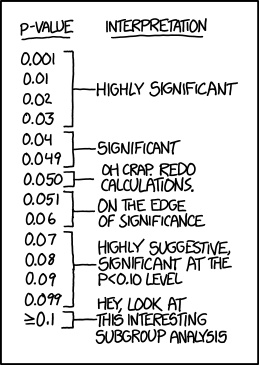
\includegraphics[width=0.6\textwidth]{p_values}
        \figcaption{xkcd:1478}
    \end{center}

\end{frame}


%%%%%
\begin{frame}{Tests and confidence intervals}

  For the $t$-test,
  \[  \text{reject $H_0$ at the $\alpha$ significance level} \]
  is \structure{equivalent to}
  \[  \text{ 0 is not in the $\alpha$-confidence interval for $\mu_1-\mu_2$ }. \]


  \vspace{2em}

  \structure{Why?}

  The $\alpha$-confidence interval asks: 
  \begin{quote}
    How big could $\mu_1-\mu_2$ be and still get a $P$-value greater than $\alpha$ for the observed $\bar y_1 - \bar y_2$?
  \end{quote}


\end{frame}


%%%%%
\begin{frame}{Example: }

    Noreprenephrin (NE) concentration (ng/gm) in rat brains:
    \begin{center}
      \begin{tabular}{c|rr}
            & Toluene & Control \\
          \hline
          $n$ & 6 & 5 \\
          $\bar y$ & 541.8 & 444.2 \\
          $s$  & 66.1 & 69.6 \\
          $\SE$ & 27 & 31 \\
     \end{tabular}
   \end{center}


     \begin{align*}
         \SE_{\bar Y_1 - \bar Y_2} &= 41.195 \\
         t_s &= 2.34  \\
         \df &= 8.47 
     \end{align*}
     $P$-value: 0.0454 .


  \vspace{2em}

  Here $t_{0.025} = 2.28$, so an $\alpha=0.05$ confidence interval is
  \[  (541.8-444.2) \pm 2.28 \times 41.195 = (3.68,191.52) . \]

\end{frame}

%%%%%
\begin{frame}{$P$-value or CI?}

  Which is better?


\end{frame}


\section<article>{Summary}
\section<presentation>*{Summary}

\begin{frame}{Summary}
  \begin{enumerate}
    \item A \structure{null hypothesis} asks if the results could be due to ``chance'';
    \item and the \structure{$P$-value} reports the probability of seeing a result at least as suprising, under that chance model.
    \item To test the null hypothesis that two groups are the same,
    \item can do a randomization test (fewer assumptions),
    \item or a $t$-test (more powerful if assumptions are met).
    \item The \structure{significance value}, $\alpha$, is the cutoff for ``significant'';
    \item it is important; but always keep in mind what the results \structure{really mean}.
    \item $\alpha$-\structure{Confidence intervals} can report the same information.
  \end{enumerate}
\end{frame}

% homework
\begin{frame}{Homework}
  \begin{center}


    7.1.2


    \vspace{2em}

    7.2.8


    \vspace{2em}

    Email me an interesting scientific study \\
    reported on in the news.

  \end{center}
\end{frame}


\end{document}





